\documentclass{article}
\usepackage{graphicx} % Required for inserting images
\usepackage{amsmath}
\usepackage{float}
\usepackage[ngerman]{babel}
\usepackage{hyperref}
\title{Abgabe 1 für Computergestützte Methoden}
\author{Gruppe 48, Carlo Möhring (4348685), Justus Thöne (4344912)}
\date{02.12.2024}

\begin{document}

\maketitle
%Inhaltsverzeichnis
\tableofcontents

\newpage
\section{Der zentrale Grenzwertsatz}
Der zentrale Grenzwertsatz (ZGS) ist ein fundamentales Resultat der Wahrscheinlichkeitstheorie, das die Verteilung von Summen unabhängiger, identisch
verteilter (i.i.d.) Zufallsvariablen (ZV) beschreibt. Er besagt, dass unter bestimmten Voraussetzungen die Summe einer großen Anzahl solcher ZV annähernd
normalverteilt ist, unabhängig von der Verteilung der einzelnen ZV. Dies ist besonders nützlich, da die Normalverteilung gut untersucht und mathematisch
handhabbar ist.

\subsection{Aussage}
Sei \(X_1, X_2, \ldots, X_n\) eine Folge von i.i.d. ZV mit dem Erwartungswert \(\mu = E(X_i)\) und der Varianz \(\sigma^2 = \text{Var}(X_i)\), wobei \(0 < \sigma^2 < \infty\) gelte. Dann konvergiert die standardisierte Summe \(Z_n\) dieser ZV für \(n \to \infty\) in Verteilung gegen eine Standardnormalverteilung:\footnote{Der zentrale Grenzwertsatz hat verschiedene Verallgemeinerungen. Eine davon ist der
\textbf{Lindeberg-Feller-Zentrale-Grenzwertsatz} \cite{Klenke2013}, Seite 328], der schwächere Bedingungen an
die Unabhängigkeit und die identische Verteilung der ZV stellt.
}
\begin{equation}
    \label{eq:standartisiert}
    \ Z_n = \frac{\sum_{i=1}^n X_i - n\mu}{\sigma \sqrt{n}} \xrightarrow{d} \mathcal{N}(0, 1).
\end{equation}
Das bedeutet, dass für große \(n\) die Summe der ZV näherungsweise normalverteilt ist mit Erwartungswert \(n\mu\) und Varianz \(n\sigma^2\):
\begin{equation}
 \label{normalverteilt}
 \sum_{i=1}^n X_i \sim \mathcal{N}(n\mu, n\sigma^2).
\end{equation}

\subsection{Erklärung der Standardisierung}
Um die Summe der ZV in eine Standardnormalverteilung zu transformieren, subtrahiert man den Erwartungswert \(n\mu\) und teilt durch die Standardabweichung \(\sigma \sqrt{n}\). Dies führt zu der obigen Formel \eqref{eq:standartisiert}. Die Darstellung \eqref{normalverteilt} ist für \(n \to \infty\) nicht wohldefiniert.
\subsection{Anwendungen}
Der ZGS wird in vielen Bereichen der Statistik und der Wahrscheinlichkeitstheorie angewendet. Typische Beispiele sind:
\begin{itemize}
    \item Durchführung von Hypothesentests
    \item Berechnung von Konfidenzintervallen für Stichprobenmittelwerte
\end{itemize}
\newpage
\section{Bearbeitung zur Aufgabe 1}
\subsection{Thema Datenverarbeitung}
\subsubsection{}In unserem Datensatz geht es um den Verleih von Fahrrädern in der E 103 St \&
Lexington Ave. Aufgebaut ist der Datensatz in die Attribute: Station, date,
precipitation, windspeed, min temperature, average temperature,
max temperature und count. Für uns sind dabei die Temperaturdaten, das Datum, sowie die Witterungsumstände von größerer Relevanz. Dabei wird
ersichtlich, dass die Anzahl der Räder stark vom Wetter und der Temperatur
abhängig ist.
\subsubsection{}Den erhaltenen Datensatz haben wir nach unserer Verleihstation gefiltert und
formatiert. Dabei haben wir die Daten etwas geordnet, indem wir die Wochentage
und Wochenzugehörigkeit entfernt haben. Da diese Informationen bereits im Datum enthalten sind.
\subsubsection{}Bei der Rechnung haben wir die Umrechnungsformel für Fahrenheit in Celsius
angewandt: (Fahrenheit – 32)*5/9. Um die größte mittlere Temperatur zu erhalten,
haben wir in Spalte J1 nach „=MAX(F2:F366)“ abgefragt und dann im nächsten Schritt
nach der Umformung ausgerechnet: SUMME =SUMME((J2)-32)*5/9. Das Ergebnis in
Grad Celsius beträgt 28,33.
\subsection{Thema Datenhaltung}
\subsubsection{Datenbank Schema} 
\begin{table}[H]
    \centering
    \begin{tabular}{|c|c|c|c|c|c|c|c|}
        \hline
        Date & Station & precipitation & windspeed & min. temp. & average temp. & max. temp. & count \\
    \hline
    \end{tabular}
    \caption{1. Normalform}
    \label{tab:my_label}
\end{table}
\begin{table}[H]
    \centering
    \begin{tabular}{|c|c|c|c|}
    \hline
ID & Date & StationID & count \\
    \hline      
    \end{tabular}
\end{table}
\begin{table}[H]
    \centering
    \begin{tabular}{|c|c|}
    \hline
StationID & Station  \\
\hline
    \end{tabular}
\end{table}
\begin{table}[H]
    \centering
    \begin{tabular}{|c|c|c|c|c|c|}
    \hline
TemperaturID & Date & StationID & min. temp. & average temp. & max. temp. \\
\hline
    \end{tabular}
\end{table}
\begin{table}[H]
    \centering
    \begin{tabular}{|c|c|c|c|c|}
    \hline
MessungenID & Date & StationID & precipitation & windspeed  \\
    \hline
    \end{tabular}
    \caption{2. Normalform}
\end{table}
\subsubsection{SQLite}
\begin{figure}[H]
    \centering
    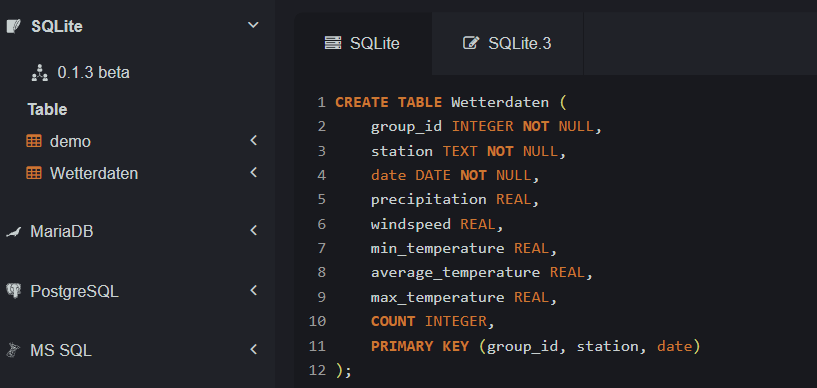
\includegraphics[scale=0.8]{SQLite 1.png}
    \caption{DDL Teil}
\end{figure}
Nachdem wir das DDL-Schema in SQLite erstellt haben, haben wir unsere CSV-Datei angepasst, um unseren Datensatz problemlos zu importieren. Dies bestand zum einen darin, dass wir die nicht benötigten Spalten wie den Tag im Jahr, den Tag der Woche oder den Monat des Jahres entfernt haben, da diese Informationen, wie oben erwähnt, bereits im Datum enthalten sind. Zusätzlich haben wir das Format des Datums in Jahr, Monat, Tag geändert, damit es mit dem Programm kompatibel wird. Anschließend haben wir die Angabe N/A aus der Spalte average temperature entfernt und sie ersetzt, damit bei der Berechnung der höchsten mittleren Temperatur nur Zahlenwerte berücksichtigt werden.
\newpage
\subsection{Abfrage in SQLite}
\begin{figure}[H]
    \centering
    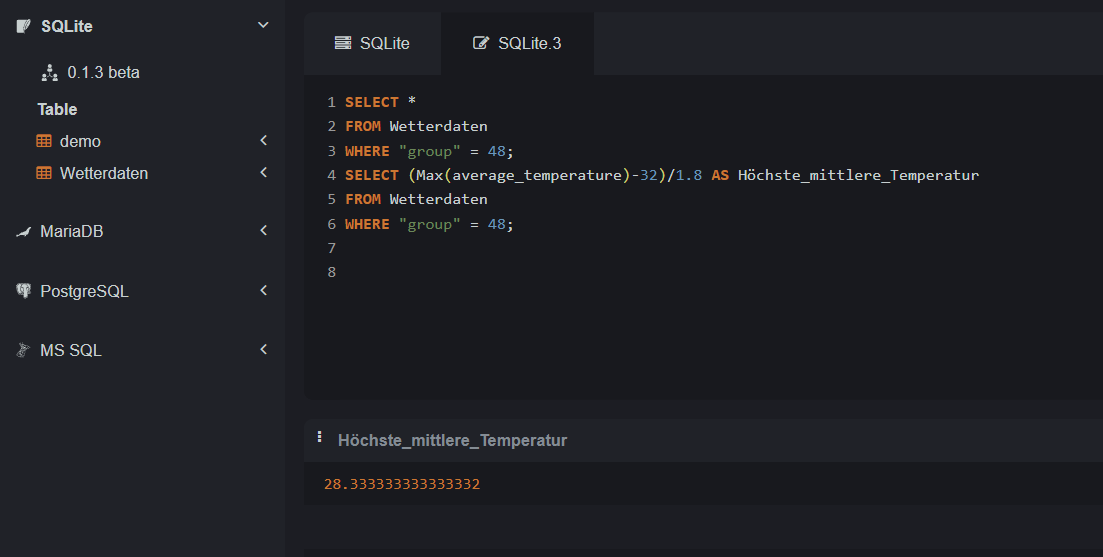
\includegraphics[scale=0.6]{SQLite 2.png}
    \caption{Abfrage in SQLite}
\end{figure}
Mithilfe des Max(average temperature) Befehls konnten wir innerhalb der Spalte nach dem größten Wert suchen. Die Formel mit -32 und /1.8 wandelt den Wert in Grad Celsius um und um nun auch nur Ergebnisse aus unserem Teil des Datensatzes anzuzeigen, wird mit where explizit die Gruppe herausgefiltert, auf welche wir uns beziehen sollen. Dies führt dazu, dass die höchste mittlere Temperatur 28,33 Grad beträgt.\\ \\ \\ \\
Link zum Repository:\url{https://github.com/CarloMoehring/CoMet-Abgabe.git}
\newpage
\bibliographystyle{plain}
\bibliography{references}
\end{document}
